\documentclass[12pt]{article}
\usepackage[utf8]{inputenc}
\usepackage{float}
\usepackage{amsmath}
\usepackage{graphicx}
\usepackage{amssymb}

\usepackage[hmargin=3cm,vmargin=6.0cm]{geometry}
%\topmargin=0cm
\topmargin=-2cm
\addtolength{\textheight}{6.5cm}
\addtolength{\textwidth}{2.0cm}
%\setlength{\leftmargin}{-5cm}
\setlength{\oddsidemargin}{0.0cm}
\setlength{\evensidemargin}{0.0cm}

%misc libraries goes here

\begin{document}

\section*{Student Information } 
%Write your full name and id number between the colon and newline
%Put one empty space character after colon and before newline
Full Name :  Alperen OVAK\\
Id Number :  2580801\\

% Write your answers below the section tags
\section*{Answer 1}

\subsection*{a)}
To determine the constant $N$ so that $P$ qualifies as a probability mass function, we need to ensure that the sum of all probabilities equals 1:

\[
\sum_{x=1}^{5} P(x) = 1
\]

Given that $P(x) = \frac{N}{x}$, the sum becomes:

\[
\frac{N}{1} + \frac{N}{2} + \frac{N}{3} + \frac{N}{4} + \frac{N}{5} = 1
\]

Now solve for $N$:

\[
N + \frac{N}{2} + \frac{N}{3} + \frac{N}{4} + \frac{N}{5} = 1
\]

\[
\frac{60N + 30N + 20N + 15N + 12N}{60} = 1
\]

\[
\frac{137N}{60} = 1
\]

\[
N = \frac{60}{137} \approx 0.438
\]

So, the constant $N$ is $\frac{60}{137}$ $\approx$ 0.438.

\subsection*{b)}
The expected value (mean) of a discrete random variable $X$ is given by:

\[
E(X) = \sum_{x} x \cdot P(x)
\]

Using the given probability mass function, we can calculate:

\[
E(X) = \sum_{x=1}^{5} x \cdot \frac{N}{x} = \sum_{x=1}^{5} N
\]

\[
E(X) = N + N + N + N + N = 5N
\]

Substitute $N = \frac{60}{137} $:

\[
E(X) = 5 \cdot \frac{60}{137} \approx 2.190
\]

\subsection*{c)}
The variance of a discrete random variable $X$ is given by:

\[
\text{Var}(X) = E(X^2) - [E(X)]^2
\]

First, calculate $E(X^2)$:

\[
E(X^2) = \sum_{x} x^2 \cdot P(x)
\]

\[
E(X^2) = \sum_{x=1}^{5} x^2 \cdot \frac{N}{x}
\]

\[
E(X^2) = \sum_{x=1}^{5} x \cdot N
\]

\[
E(X^2) = N + 2N + 3N + 4N + 5N = 15N
\]

Now, calculate the variance:

\[
\text{Var}(X) = 15N - (5N)^2
\]

Substitute $N = \frac{60}{137}$, we get:

\[
\text{Var}(X) \approx 1.774
\]

\subsection*{d)}
For the joint distribution, $P(x, y) = P(x)P(y)$. Calculate $E(XY)$, $E(X)$, and $E(Y)$ to find the covariance:

\[
E(XY) = \sum_{x}\sum_{y} xy \cdot P(x, y)
\]

\[
E(XY) = \sum_{x=1}^{5}\sum_{y=1}^{5} xy \cdot P(x)P(y)
\]

\[
E(XY) = \sum_{x=1}^{5}\sum_{y=1}^{5} xy \cdot \frac{N}{x} \cdot \frac{y}{15}
\]

\[
E(XY) =  \sum_{x=1}^{5}\sum_{y=1}^{5} \frac{N}{15} \cdot y^2
\]


\[
E(XY) \approx 8.029
\]

Note that $E(X)E(Y) =8.030 $. Since $E(X)E(Y) \approx E(XY)$, we can say that X and Y is independent. \\

Now, calculate $E(X)$ and $E(Y)$ using the results from parts b) and c). Finally, use the formula $\text{Cov}(X, Y) = E(XY) - E(X)E(Y)$ to find the covariance. Interpret the covariance value in terms of the relationship between $X$ and $Y$. \\

$\text{Cov}(X, Y) = E(XY) - E(X)E(Y) = 0$


\section*{Answer 2}

\subsection*{a)} 

Let $p$ be the probability of success in a single attempt. The probability of failure in a single attempt is $1 - p$.

The probability of not having a success in a single attempt is $1 - p$. The probability of not having a success in all 1000 attempts is $(1 - p)^{1000}$.

Now, the probability of at least one success in 1000 attempts is the complement of the probability of no success in all attempts:

\[
P\{X \geq 1\} = 1 - P\{X \leq 1\}
\]

Given that the probability of no success in a single attempt is $(1 - p)$, the probability of no success in all 1000 attempts is $(1 - p)^{1000}$.

So, we want to find $p$ such that:

\[
1 - (1 - p)^{1000} = 0.95
\]

Now, we can solve this equation for $p$:

\[
(1 - p)^{1000} = 0.05
\]

Taking the 1000th root of both sides:

\[
1 - p = 0.05^{1/1000}
\]

Now, solve for $p$:

\[
p = 1 - 0.05^{1/1000}
\]

Calculating this gives the probability of success for an individual attempt:

\[
p \approx 0.003
\]

So, the probability of success for an individual attempt should be approximately $0.003$ to ensure that the probability of at least one success in 1000 trials is 95%.


\subsection*{b)} 
\textbf{i)}
Let \( X \) be the number of games played until 2 matches are won against
an IM for an average player. Since \( X \) has Negative Binomial distribution with \( k = 2\) and \( p = 0.003 \), it is a number of trials needed to see 2 won. We need \( P\{X > 500\} = \sum_{n=501}^{\infty} P(x) \) or \( 1 - F(500) \); however, there is no table of Negative Binomial distribution in the Appendix, and applying the formula for \( P(x) \) directly. \\
Instead, we can solve this problem by a Binomial distribution. Although \( X \) is not Binomial at all, the probability \( P\{X > 500\} \) can be related to some Binomial variable.

\begin{align*}
P\{X > 500\} &= P\{ \text{more than 500 games needed to get 2 won} \} \\
            &= P\{ \text{500 games are not sufficient} \} \\
            &= P\{ \text{there are fewer than 2 wons in 500 games} \} \\
            &= P\{Y < 2\} ,
\end{align*}
where \( Y \) is the number of successes (non-defective components) in 500 games, which is a Binomial variable with parameters \( n = 500 \) and \( p = 0.003 \).
\[ P\{X > 500\} = P\{Y < 2\} = P\{Y \leq 1\} = F(2) \]

We can calculate this as follows:

\[ F(2) = P(0) + P(1) \]

According to the Binomial distribution formula $P(x) = P\{X = x\} = \binom{n}{x} p^x q^{n-x}$:

\begin{align*}
P(0) &=   \binom{500}{0} p^0 q^{500-0}\\
     &=   1 \times (0.003)^0 \times (1-0.003)^{500-0} \\
     &=   1 \times 1 \times (0.997)^{500} \\
     &=   (0.997)^{500} \\
     &\approx   0.223\\
\end{align*}

\begin{align*}
P(1) &=   \binom{500}{1} p^1 q^{500-1}\\
     &=   500 \times (0.003)^1 \times (1-0.003)^{500-1} \\
     &=   500 \times (0.003) \times (0.997)^{499} \\
     &\approx   0.335\\
\end{align*}

Therefore, Our answer is:

\[ F(2) \approx 0.223 + 0.335 \approx 0.558\]

\textbf{ii)} This question is very similar to above question. We can solve it in same way:

\begin{align*}
P\{X > 10^4\} &= P\{ \text{more than $10^4$ games needed to get 2 won} \} \\
            &= P\{ \text{$10^4$ games are not sufficient} \} \\
            &= P\{ \text{there are fewer than 2 wons in $10^4$ games} \} \\
            &= P\{Y < 2\} ,
\end{align*}

Solve by Binomial variable with parameters \( n = 10^4 \) and \( p = 10^{-4} \).
\[ P\{X > 10^4\} = P\{Y < 2\} = P\{Y \leq 1\} = F(2) \]

\[ F(2) = P(0) + P(1) \]

\begin{align*}
P(0) &=   \binom{10^4}{0} p^0 q^{10^4-0}\\
     &=   1 \times (10^{-4})^0 \times (1-10^{-4})^{10^4-0} \\
     &=   1 \times 1 \times (1-10^{-4})^{10^4} \\
     &=   (1-10^{-4})^{10^4} \\
     &=   0.367861046\\
\end{align*}

\begin{align*}
P(1) &=   \binom{10^4}{1} p^1 q^{10^4-1}\\
     &=   10^4 \times (10^{-4})^1 \times (1-10^{-4})^{10^4-1} \\
     &=   0.367897836\\
\end{align*}

Therefore, Our answer is:

\[ F(2) \approx 0.367861046 + 0.367897836 \approx 0.7358\]

\subsection*{c)} 

Let \( X \) be the number of days feeled healthy. It is the number of successes in 366 Bernoulli trials, thus \( X \) is Binomial with \( n = 366 \) and \( p = 0.98 \). Poisson approximation cannot be applied to \( X \) because \( p \) is too large. However, the number of failures \( Y \) is also Binomial, with parameters \( n = 366 \) and \( q = 0.02 \), and it is approximately Poisson with \( \lambda = nq = 7.32 \). \\

From Table A3, there is no value for $\lambda =7.32 $. Thus, we need to choose most fitting values from Table A3 which is $\lambda =7.5 $
\[ P \{X \geq 360\} = P \{Y \leq 6\} = F_Y(6) \approx 0.378. \]


\section*{Answer 3}
\subsection*{a)} 
\begin{figure}[h]
    \centering
    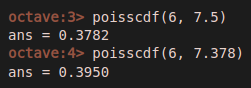
\includegraphics{3a_kod}
    \caption{CDF of the Poisson distribution for different values of lambda with the same number of events}
\end{figure}

The Poisson CDF represents the probability that the number of events in a Poisson process will be less than or equal to a certain value. So, in this case, we're comparing the probabilities of observing 6 or fewer events in two Poisson distributions with different lambda values. \\

In the Poisson distribution, the parameter $\lambda$ represents the average rate of occurrence of events in a fixed interval. In this case, we're comparing two scenarios where the average rate of occurrence is slightly different: $\lambda_1 = 7.32$ and $\lambda_2 = 7.5$. \\

To compare the two cumulative probabilities:

\begin{itemize}
    \item $\text{poisscdf}(6, 7.32)$: This represents the probability of observing 6 or fewer events in a Poisson process with an average rate of occurrence of $\lambda_1 = 7.32$.

    \item $\text{poisscdf}(6, 7.5)$: This represents the probability of observing 6 or fewer events in a Poisson process with an average rate of occurrence of $\lambda_2 = 7.5$.
\end{itemize}

Since the average rate of occurrence $\lambda_2 = 7.5$ is slightly higher than $\lambda_1 = 7.32$, it implies that there's a slightly higher chance of observing more events in the process with $\lambda_2$ compared to $\lambda_1$. Therefore, the cumulative probability of observing 6 or fewer events in the process with $\lambda_2$ ($\text{poisscdf}(6, 7.5)$) will be lower than the cumulative probability in the process with $\lambda_1$ ($\text{poisscdf}(6, 7.32)$).

Thus, the higher the average rate of occurrence ($\lambda$), the more spread out the Poisson distribution becomes, resulting in a higher probability of observing larger numbers of events, which is reflected in the cumulative distribution function.


\subsection*{b)} 

\begin{figure}[H]
    \centering
    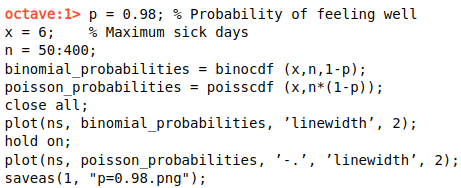
\includegraphics[scale=0.6]{3b_kod}
    \caption{The code of Poisson and Binomial probabilities for p=0.98}
\end{figure}

\begin{figure}[H]
    \centering
    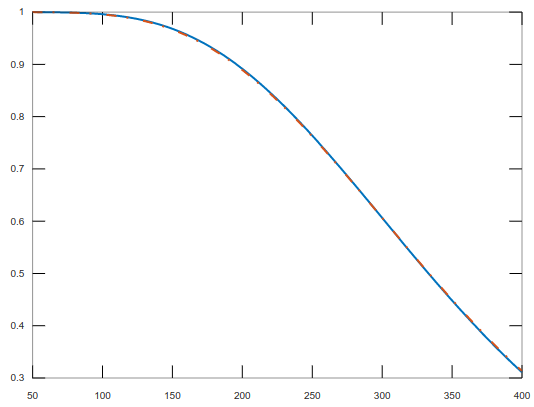
\includegraphics[scale=0.5]{3b_graph}
    \caption{The graph of Poisson and Binomial probabilities for p=0.98}
\end{figure}

\subsection*{c)} 

\begin{figure}[H]
    \centering
    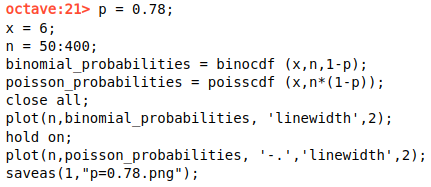
\includegraphics[scale=0.6]{3c_cod}
    \caption{The code  of Poisson and Binomial probabilities for p=0.78}
\end{figure}

\begin{figure}[H]
    \centering
    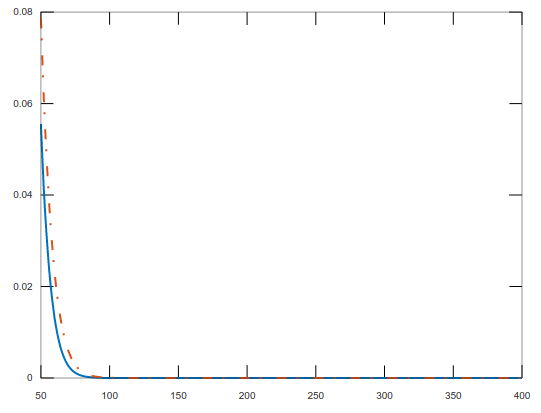
\includegraphics[scale=0.5]{3c_graph}
    \caption{The graph of Poisson and Binomial probabilities for p=0.78}
\end{figure}

According to Chapter 3.4.6, The Poisson distribution is a suitable approximation for binomial probabilities when there are a large number of trials (n) and a small probability of success (p). This approximation is acceptable for cases where n $\geq$ 30 and p $\leq$ 0.05. As n increases, the accuracy of this approximation improves.\\

In the first example, since our p  $ = 1-0.98 = 0.02 \leq 0.05 $ for Poisson distribution, the condition ensure that np, which represents the mean of the Binomial distribution is moderate enough for the Poisson approximation to hold. This parallel result aligns with the Binomial distribution (Figure 3).\\

On the other hand, in the second example, since our p  $ = 1-0.78 = 0.22  \nless 0.05 $, the Poisson approximation of the Binomial distribution becomes less accurate due to violations of the assumptions underlying the approximation. In this scenario, the assumptions for using the Poisson distribution as an approximation of the Binomial distribution does not hold (Figure 5).\\

\end{document}
